\documentclass[12pt]{article}

\usepackage[english]{babel}
\usepackage[utf8x]{inputenc}
\usepackage[T1]{fontenc}
\usepackage{parskip}
\usepackage{lipsum}
\usepackage[a4paper, total={6in, 8in}]{geometry}
\usepackage{setspace}
\usepackage[superscript]{cite}
\usepackage{xcolor}
\usepackage{hyperref}
\usepackage{enumitem}
\usepackage{listings}
\usepackage{amsmath}
\usepackage{amssymb}
\usepackage{ifsym}
\usepackage{tikz}


\begin{document}
	
	
	\begin{flushright}
		\today
	\end{flushright}
	{\Large \textbf{Assignment 11}}
	
	{\large Query Optimization}
	
	\textsc{Ilaria Battiston - 03723403} \\
	\textsc{Mareva Zenelaj - 03736071}
	
	\rule{\linewidth}{0.5pt}
	
	\section{First exercise}
	
	$m = 3$ 
	
	$n = 2$ 
	
	$N = m * n = 6$ 
	
	$k = 2$ 
	
	$p = \frac{\binom{N - k}{k}}{\binom{N}{k}} = \frac{\binom{4}{2}}{\binom{6}{2}} = \frac{6}{15}$
	
	$\overline{{Yao}}_n^{N,m} (k) = m * {Yao}_n^N (k)$
	
	since $k \leq N - n$ then ${Yao}_2^6 (2) = 1 - p = 1 - 0.4 = 0.6$
	
	$\overline{{Yao}}_2^{6,3} (2) = 3 * 0.6 = 1.8$
	
	\section{Second exercise}
	
	$m = 3$ 
	
	$n = 2$ 
	
	$N = m * n = 6$ 
	
	$k = 4$ 
	
	Since the tuples are not necessarily distinct, we use Cheung's formula. 
	
	$\overline{{Cheung}}_n^{N,m} (k) = m * {Cheung}_n^N (k)$
	
	where 
	
    ${Cheung}_n^N (k) = [1-\tilde{p}]$
    
    and $\tilde{p} = \prod_{i=0}^{k-1} \frac{N-n+i}{N+i}$
    
    $\tilde{p} = \prod_{i=0}^{3} \frac{4+i}{6+i} = \frac{4}{6} * \frac{5}{7} * \frac{6}{8} * \frac{7}{9} = 0.278$
    
    $\overline{{Cheung}}_2^{6,3} = 3 * (1 - 0.278) = 2.167 $
    
    \section{Third exercise}
    
    \begin{center}
    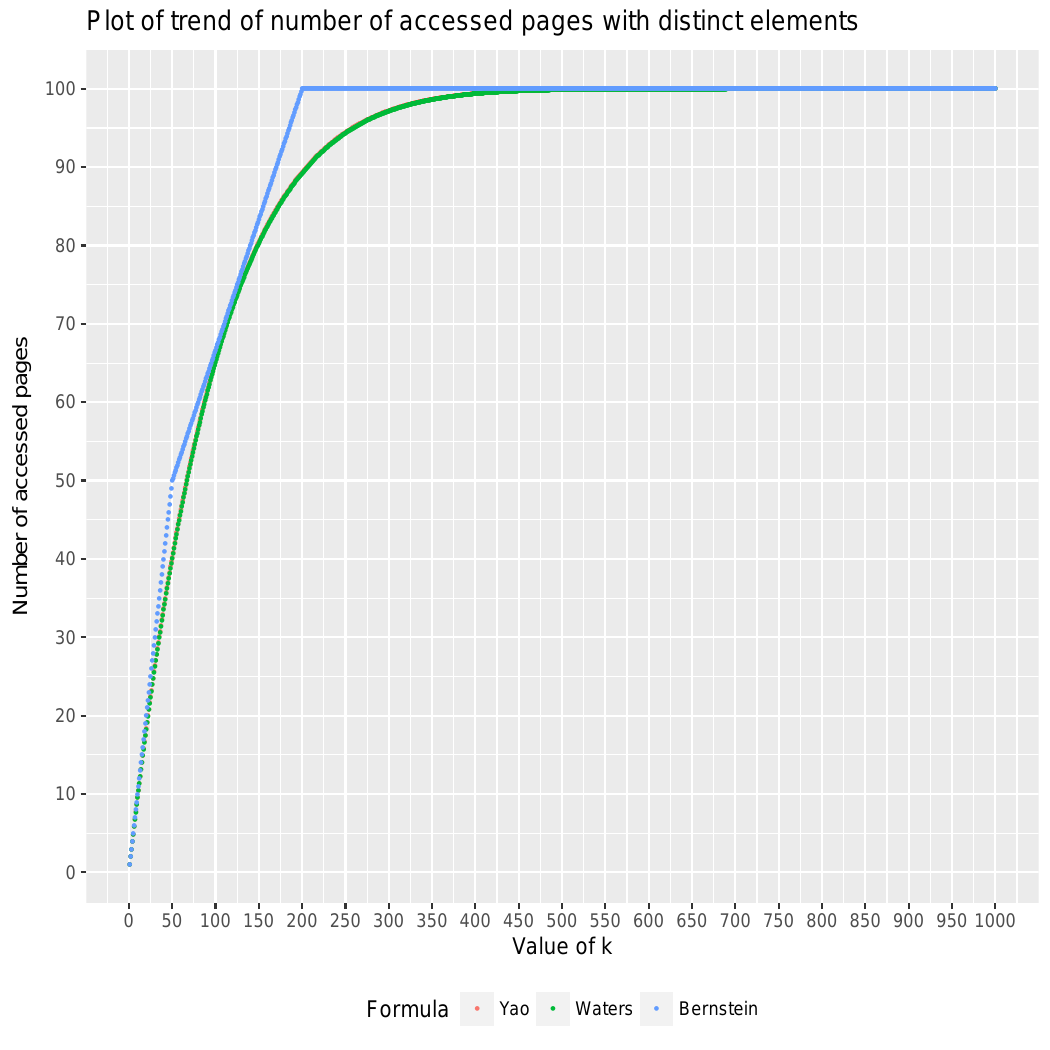
\includegraphics[width=\textwidth]{yao_bernstein_waters.png}
    \end{center}
    
    Yao and Waters (red and green) results overlap in the graph.
    
    \section{Fourth exercise}
    
    \begin{center}
    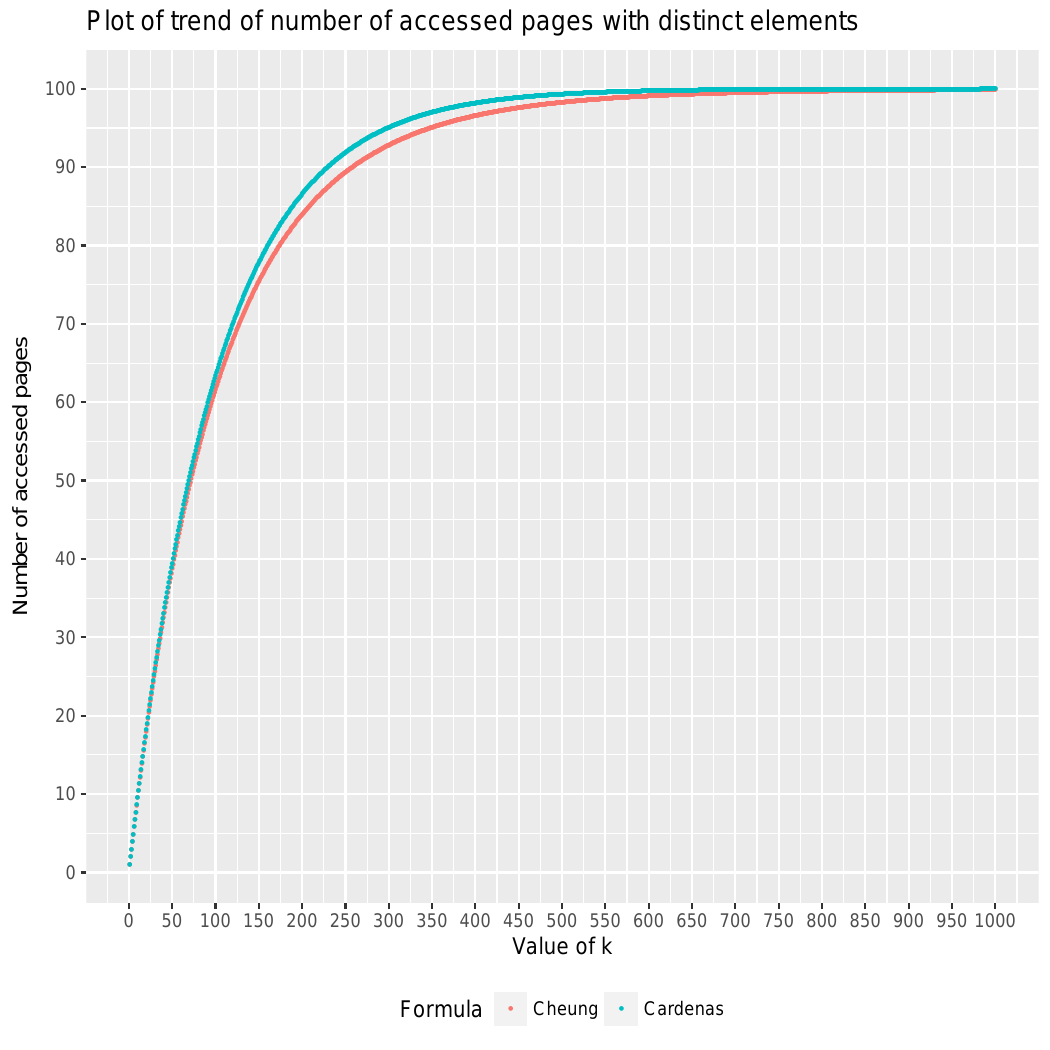
\includegraphics[width=\textwidth]{cheung_cardenas.png}
    \end{center}
    
    Below we include all results together:
    \begin{center}
    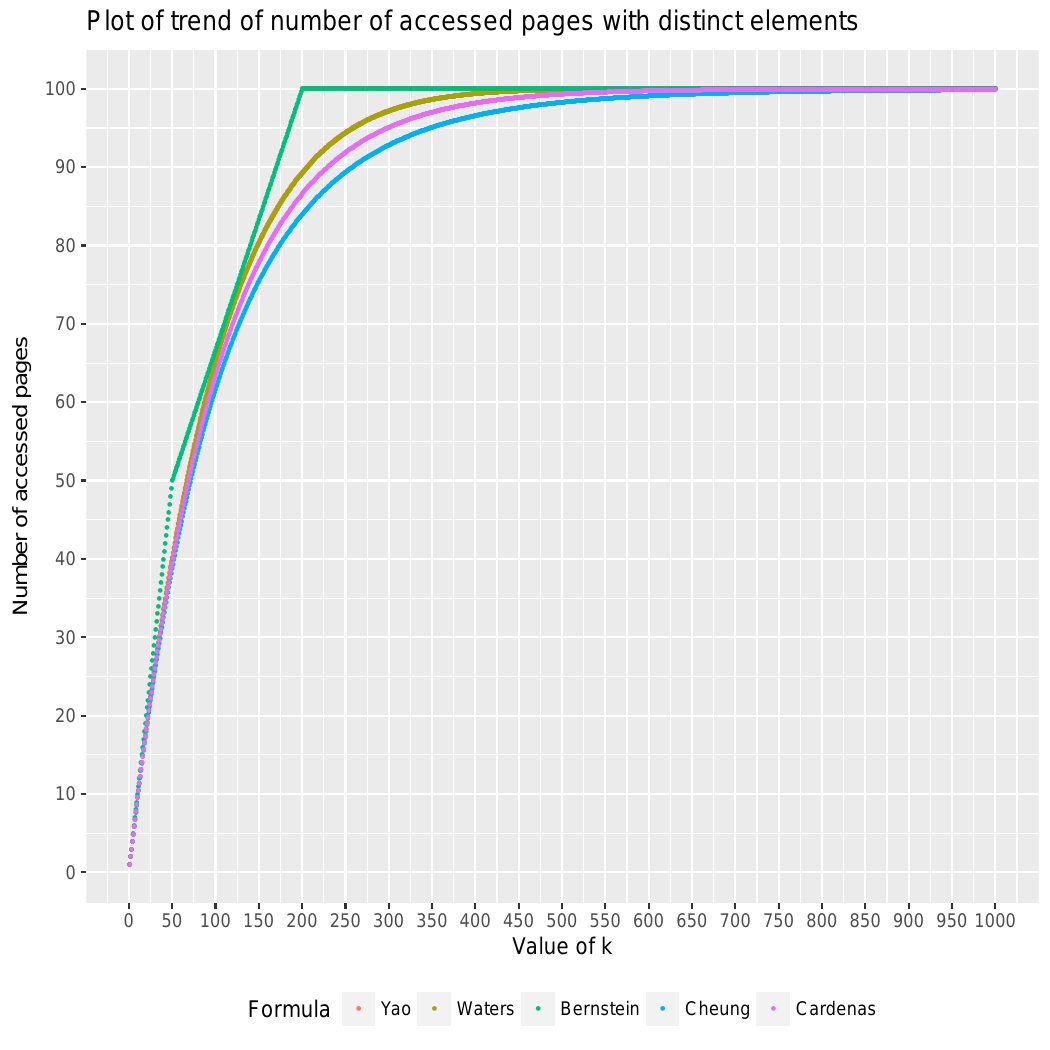
\includegraphics[width=\textwidth]{all_approx.png}
    \end{center}
    
\end{document}